%! TeX root = report.tex

\section{Spec 4b: Further abstractions}

Disappointed with the results in Section~\ref{sec:spec4}, we have decided to
push abstractions even further. These abstractions helped us to verify
accountable safety for the configuration in Figure~\ref{fig:three}.
Unfortunately, they do not scale to larger configurations. In any case, we
find these abstractions quite important for further research on model checking
of algorithms similar to 3SF\@.

\subsection{Constraints over set cardinalities}

\SpecThree{} contains several comparisons over set cardinalities. For example:

\begin{equation}
    3 * \textit{Cardinality}(\textit{validatorsWhoCastJustifyingVote}) \ge 2 \cdot N
    \label{eq:card-comparison}
\end{equation}

In the general case, the symbolic model checker has to encode constraints for
the cardinality computation in Equation~(\ref{eq:card-comparison}). If a set
$S$ contains up to $n$~elements, Apalache produces $O(n^2)$~constraints for
$\textit{Cardinality(S)}$.

To partially remediate the above issue in~\SpecFour{}, we introduce a
constant~$T$ for the upper bound on the number of faulty process, and further
refine Equation~(\ref{eq:card-comparison}) to:

\begin{equation}
    \textit{Cardinality}(\textit{validatorsWhoCastJustifyingVote}) \ge 2 \cdot T + 1
    \label{eq:card-comparison2}
\end{equation}

Apalache applies an optimized translation rule for
Equation~(\ref{eq:card-comparison2}). Essentially, the solver has to find $2
\cdot T + 1$ set elements to show that Equation~(\ref{eq:card-comparison2})
holds true. This gives us a linear number of constraints, instead of a
quadratic one. For example, when $T=1$ and the set may contain up to~$n$
elements, the model checker produces $3 \cdot O(n)$ constraints to check
Equation~(\ref{eq:card-comparison2}). A similar optimization is used in the
specification of Tendermint~\cite{TendermintSpec2020}.

\subsection{Quorum sets}

To further optimize the constraints over set cardinalities, we have applied the
well-known pattern of replacing cardinality tests with quorum sets. For
example, this approach is used in the specification of Paxos\footnote{%
    \tlap{} specification of Paxos:
\url{https://github.com/tlaplus/Examples/blob/master/specifications/Paxos/Paxos.tla}.}

To this end, we introduce quorum sets such as in Figure~\ref{fig:quorum-sets}.

\begin{figure}[!h]
    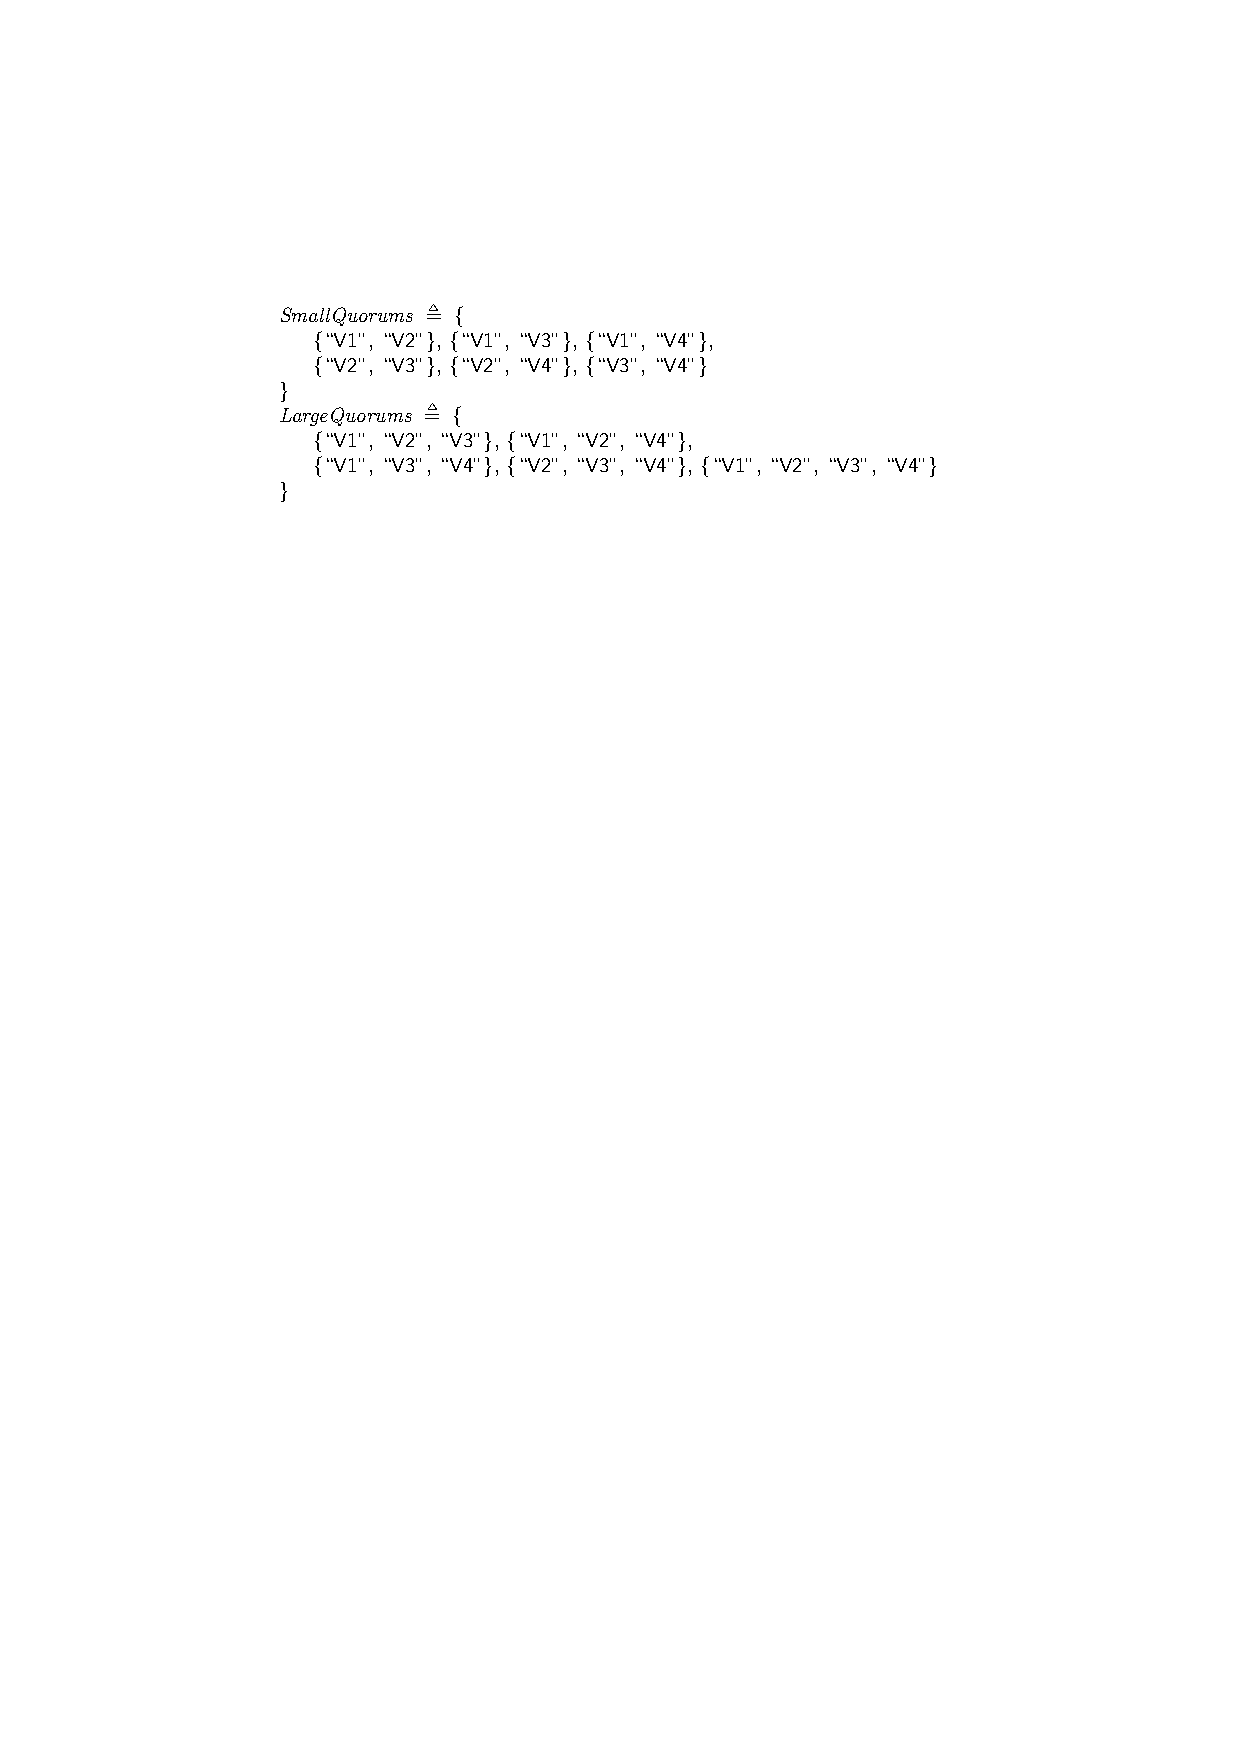
\includegraphics[width=\textwidth]{images/quorum-sets}
    \caption{Quorum sets}\label{fig:quorum-sets}
\end{figure}

By using quorum sets, we further replace cardinality comparisons like in
Equation~(\ref{eq:card-comparison2}) with membership tests like in
Equation~(\ref{eq:card-comparison3}):

\begin{equation}
    \textit{validatorsWhoCastJustifyingVote} \in \textit{LargeQuorums}
    \label{eq:card-comparison3}
\end{equation}


\subsection{Decomposition of chain configurations}\label{sec:decomposition}

Recall Figure~\ref{figFork} from Section~\ref{sec:spec4-indinv}, which poses
constraints on the chains and the fork points. While these constraints should
be easier for an SMT solver than general reachability properties, they
still produce a number of arithmetic constraints. On the other hand, when we do
model checking for small parameters, there is a relatively small set of
possible chain configurations.  Figure~\ref{fig:block-graphs} shows some of
these configurations for the graphs of 3 to 7 blocks.

This observation led us to the following idea. Instead of using the constraints
over blocks such as in Figure~\ref{figFork}, we introduce one instance per
chain configuration. It is thus sufficient to verify accountable safety for all
of these instances and aggregate the model checking results.

Figure~\ref{fig:indinit-c3} shows an initialization predicate for the
configuration shown in Figure~\ref{fig:five2}. This predicate replaces the
general initialization predicate that we discussed in
Section~\ref{sec:spec4-indinv}.

\begin{figure}
    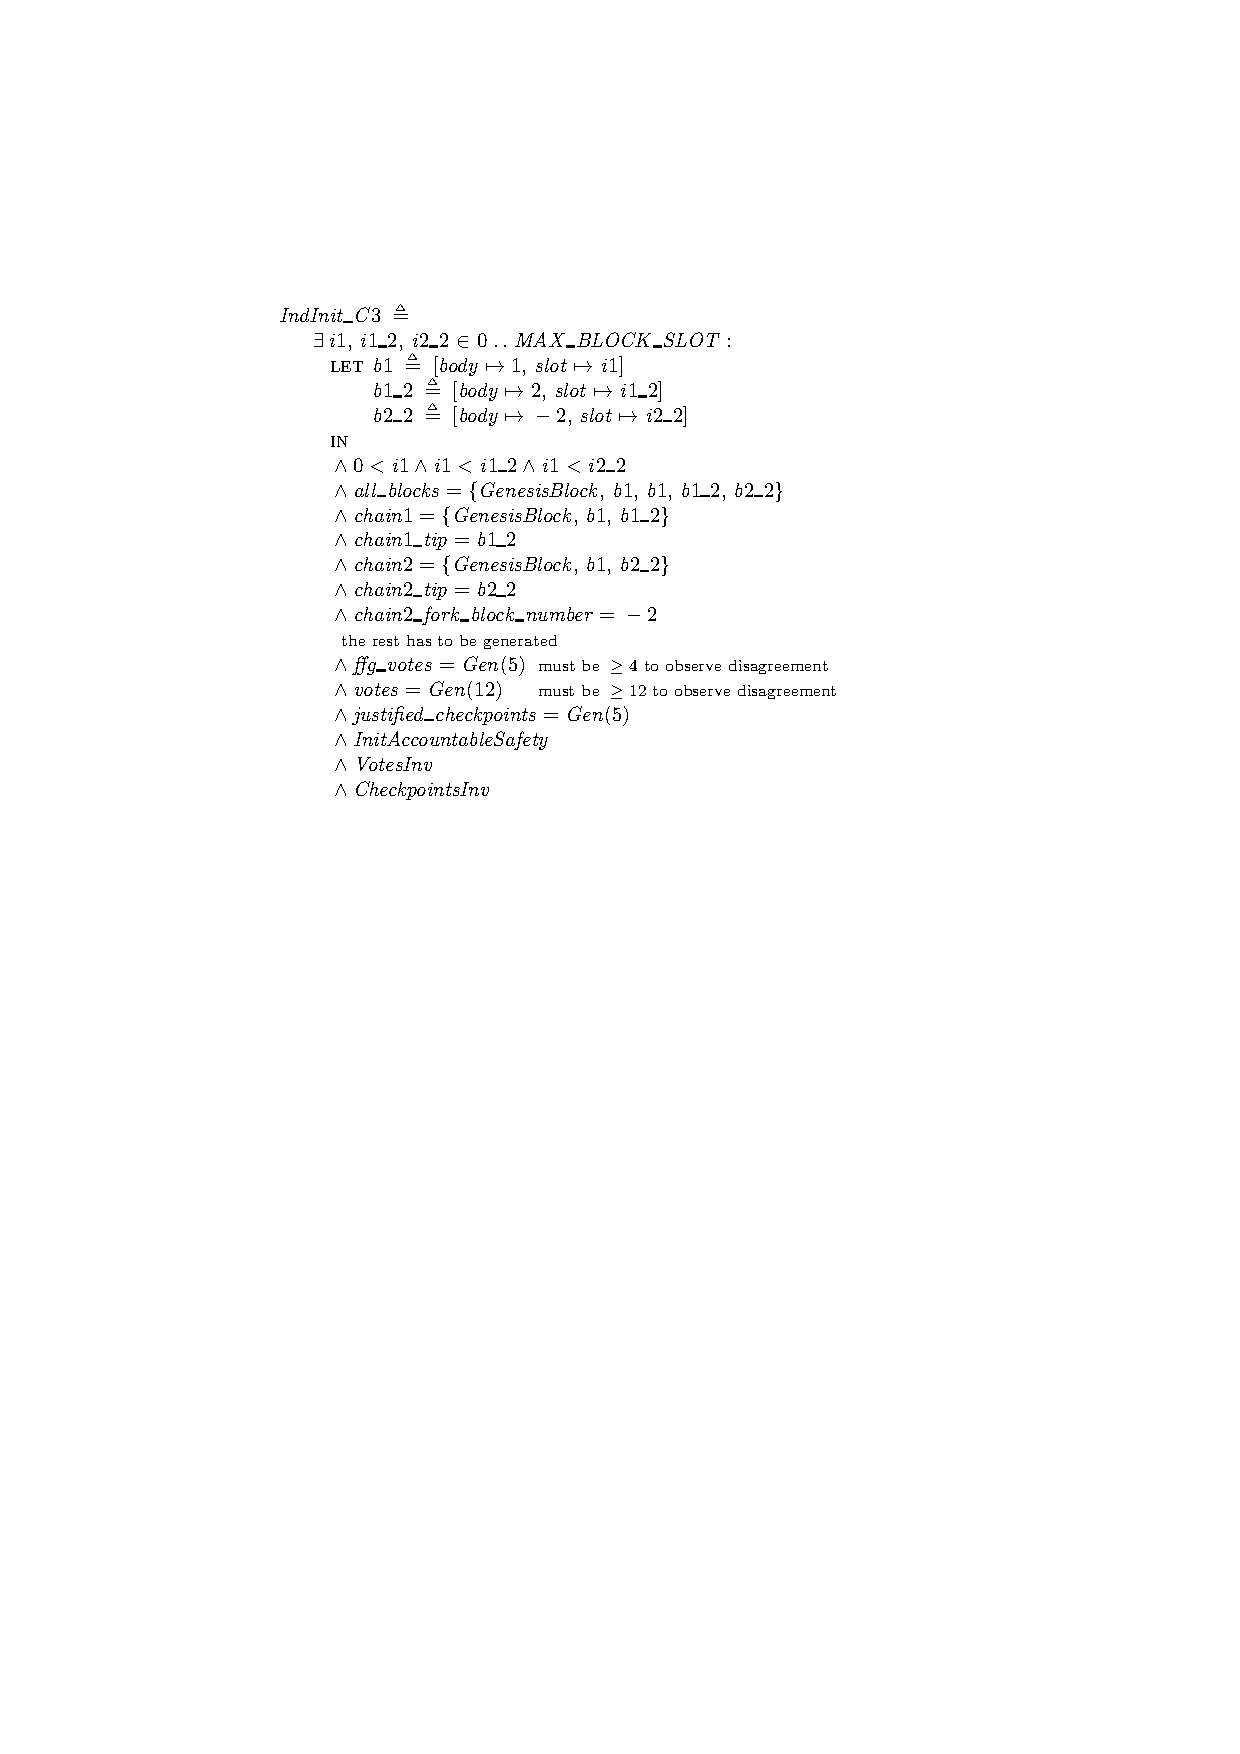
\includegraphics[width=\textwidth]{images/indinit-c3}
    \caption{Initialization predicate for the
             configuration~\text{M5b}}\label{fig:indinit-c3}
\end{figure}

\subsection{Model checking experiments}

Table~\ref{tab:spec4b-experiments} summarizes our experiments with Apalache for
various configurations. One interesting effect of the optimizations,
especially of the ones presented in Section~\ref{sec:decomposition}, is
a significant drop in the memory consumption of the SMT solver. In our
experiments, Z3 required from 700~MB to 1.5~GB\@. While this is still a factor of
20 in comparison to the Alloy experiments in Section~\ref{sec:alloy}, this is
significantly better than our initial experiments with~\SpecTwo{}
and~\SpecThree{}, which required up to 20~GB of RAM\@.

\begin{table}
    \centering
    \begin{tabular}{lrr}
        \tbh{Configuration}
            & \tbh{Memory}
            & \tbh{Time}
            \\ \toprule
        M3: Fig.~\ref{fig:three}
            & XXX
            & XXX
            \\
        M4a: Fig.~\ref{fig:four-top}
            & XXX
            & XXX
            \\
        M4b: Fig.~\ref{fig:four-bottom}
            & XXX
            & XXX
            \\
        M5a: Fig.~\ref{fig:five1}
            & XXX
            & XXX
            \\
        M5b: Fig.~\ref{fig:five2}
            & XXX
            & XXX
            \\
            \bottomrule
    \end{tabular}
    \caption{Model checking experiments with Spec 4b}\label{tab:spec4b-experiments}
\end{table}

